%==============================================================================
\chapter{SURVEY}\label{sec:5}
%==============================================================================

%==============================================================================
Neste capítulo informações mais detalhadas são apresentadas sobre o levantamento (\textit{survey}) que foi conduzido. 
Na \Cref{sec:survey-protocol}, é apresentado detalhes sobre o protocolo adotado, autor de referencia e divisão de tarefas entre os pesquisadores. 
Logo na \Cref{sec:survey-threats}, as ameaças a validade do estudo são relatadas, e por fim na \Cref{sec:survey-results}, todos os resultados alcançados durante a execução são discorridos.

%==============================================================================

\section{Survey Protocol} \label{sec:survey-protocol}

%==============================================================================
Um levantamento (\textit{survey}) é uma abordagem de coleta e análise de dados em que os participantes respondem a perguntas ou a declarações que foram desenvolvidas antecipadamente. 
O protocolo escolhido para a elaboração desta pesquisa foi inspirado nas diretrizes propostas por \citeonline{kasunic2005designing}, em \textit{Designing an effective survey} e está ilustrado na \Cref{fig:setepassos}.

%==============================================================================

\begin{figure}[htb]
  \caption{Seven steps of the research process}\label{fig:setepassos}
  \begin{center}
    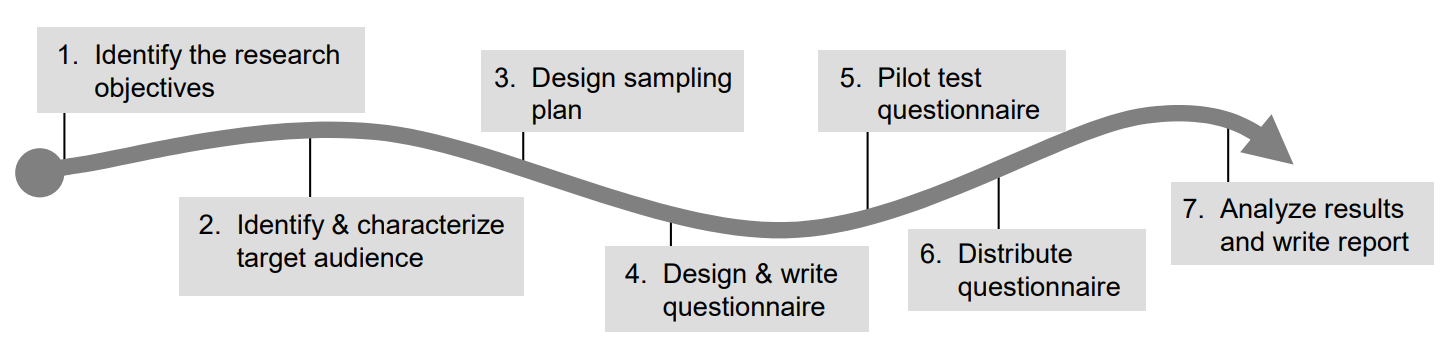
\includegraphics[width=16cm]{img/kasunic_process.png}
  \end{center}
  \fonte{\cite{kasunic2005designing}.}
\end{figure}

%==============================================================================
Como será dito posteriormente, o objetivo é compreender as necessidades de discentes e docentes em relação aos projetos e atividades de extensão. 
A escolha do \textit{survey} como abordagem de coleta de dados se deve ao fato de que as características de uma pesquisa deste tipo nos permite generalizar sobre as crenças e opiniões de muitas pessoas estudando apenas um subconjunto delas \cite{kasunic2005designing}. 
Sendo, neste caso, a ferramenta ideal.

%==============================================================================

%==============================================================================
Tendo em vista que esta pesquisa foi executada por dois estudantes, a carga de trabalho foi dividida, de maneira que a qualidade e desempenho fossem melhorados. 
Na \Cref{tbl:survey-tasks} se encontra a divisão de atividades adotada, contemplando as já definidas por \citeonline{kasunic2005designing}.

%==============================================================================

% Tabela \Cref{tbl:survey-tasks} Activity Division
\begin{table}[!htb]
  \centering
  \caption{Tasks Separation}
  \label{tbl:survey-tasks}
  \footnotesize
  \begin{tabular}{l|l}
    \bottomrule
    \rowcolor[rgb]{0.753,0.753,0.753} \multicolumn{1}{c|}{\textbf{Activity}}                             & \multicolumn{1}{c}{\textbf{Responsibility}} \\
    \hline
    \rowcolor[rgb]{0.898,0.898,0.898} Define and document research objectives                            & Lucas F.                                    \\
    Define and document research questions                                                               & Lucas F.                                    \\
    \rowcolor[rgb]{0.898,0.898,0.898} Define and document how research results will be used              & Lucas F.                                    \\
    Define the appropriate target audience for the research                                              & Igor C.                                     \\
    \rowcolor[rgb]{0.898,0.898,0.898} Determine the appropriate media to apply the research in           & Igor C.                                     \\
    Recruit members of the target audience to participate in pilot test                                  & Igor C.                                     \\
    \rowcolor[rgb]{0.898,0.898,0.898} Breakdown research questions into questionnaire topics             & Lucas F.                                    \\
    Organize and sequence questions                                                                      & Lucas F.                                    \\
    \rowcolor[rgb]{0.898,0.898,0.898} Review the questionnaire based on the pilot test                   & Igor C. and Lucas F.                        \\
    Perform the pilot test                                                                               & Igor C. and Lucas F.                        \\
    \rowcolor[rgb]{0.898,0.898,0.898} Evaluate comments                                                  & Igor C. and Lucas F.                        \\
    Perform final corrections before the distribution of the questionnaire                               & Lucas F.                                    \\
    \rowcolor[rgb]{0.753,0.753,0.753} \multicolumn{1}{c|}{\textbf{Questionnaire ready for distribution}} &                                             \\
    Distribute questionnaires                                                                            & Lucas F.                                    \\
    \rowcolor[rgb]{0.898,0.898,0.898} Monitor answers                                                    & Igor C. and Lucas F.                        \\
    Send reminders                                                                                       & Igor C.                                     \\
    \rowcolor[rgb]{0.753,0.753,0.753} \multicolumn{1}{c|}{\textbf{Questionnaire response deadline}}      &                                             \\
    Perform analysis                                                                                     & Igor C. and Lucas F.                        \\
    \rowcolor[rgb]{0.898,0.898,0.898} Write draft report                                                 & Igor C.                                     \\
    Revise draft                                                                                         & Igor C. and Lucas F.                        \\
    \rowcolor[rgb]{0.898,0.898,0.898} Perform the final corrections                                      & Igor C. and Lucas F.                        \\
    \toprule
  \end{tabular}
\end{table}

\subsection{Identify the Research Objectives} \label{sec:survey-objectives}
% Objetivo do survey -> refinamento dos requisitos, validar, importancia
% Transformar em uma questão de pesquisa, pergunta
% grey gerou resultados pra usar no survey com o olhar dos futuros usuarios

%==============================================================================
O objetivo deste primeiro passo é identificar qual a importância e o por que de fazer um survey, o que poderia ser conquistado com ele.
Levando em conta os resultados gerados pela revisão na literatura cinza, mencionados no \Cref{grey_literature}, foi possível elaborar questões de maneira que o participante informe, na sua visão, a importância de determinado requisito levantado. 
Logo, o objetivo deste survey é ordená-los por prioridade, utilizando a opinião de possíveis usuários finais.
%==============================================================================

%==============================================================================
Além de ser perguntado a opinião dos participantes, foi permitido com que eles fornecessem sugestões ou melhorias em relação a requisitos da ferramenta, já que um dos objetivos da pesquisa está voltado a entender as necessidades dos possíveis usuários do sistema. 
Assim, tendo uma base mais sólida para começar o processo de desenvolvimento da solução corretamente, com os escopos das atividades mais bem definidos.

%==============================================================================
\subsection{Identify and Characterize the Target Audience} \label{sec:survey-targets}
%==============================================================================
Neste estágio, é necessário olhar para os possíveis públicos respondentes e identificar quem será o público respondente e quem é a população do estudo. Assim sendo, a população é composta por todos as pessoas dentro da comunidade acadêmica, logo foi escolhido para representarem a amostra desta população os coordenadores de programas ou projetos de extensão, docentes e discentes, tendo preferência em participantes que tenham experiência com atividades de extensão. Com este público é possível ter o ponto de vista de todos os usuários da ferramenta, quem cria atividades e quem se inscreve em uma.
%==============================================================================
% Para possívelmente conseguir melhores sugestões nas respostas do survey, foi necessário abrangir a maior quantidade de campus da \ac{UNIPAMPA} possivel, era esperado que campus como Uruguaiana, Bagé e Dom Pedrito que, como visto na \Cref{fig:number-of-projects} foram os campus que mais possuiram atividades de extensão no ano de 2017 de acordo com \cite{relatorio-2017}, fornecessem mais respondentes, mas no final isto nao aconteceu.

% \begin{figure}[htb]
%   \caption{Number of Projects Contemplated in the Internal Public Notices}\label{fig:number-of-projects}
%   \begin{center}
%     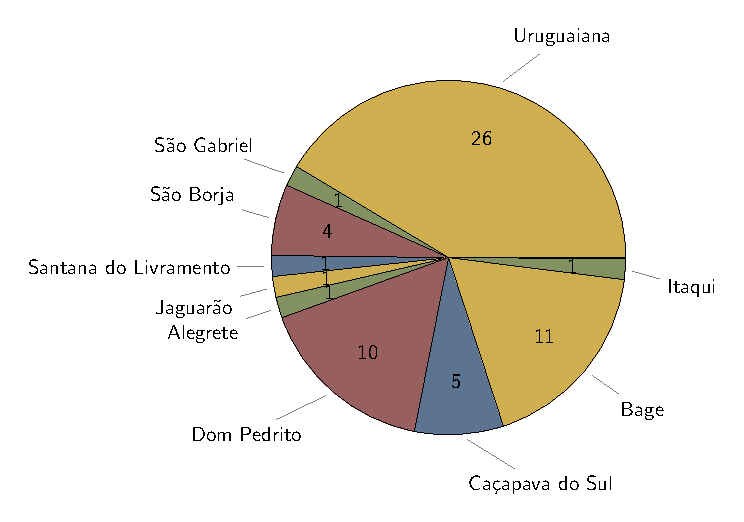
\includegraphics[width=16cm]{img/uruguaiana.pdf}
%   \end{center}
%   \fonte{Adapted from \cite{relatorio-2017}}
% \end{figure}

\subsection{Design the Sampling Plan} \label{sec:survey-sampling}

%==============================================================================
De acordo com \citeonline{kasunic2005designing}, o objetivo desta fase é determinar os seguintes tópicos:
\begin{itemize}
    \item How individuals will be selected to participate in the survey;
    \item The required size of the sample.
\end{itemize}
%==============================================================================

%==============================================================================
Por isso, o primeiro tópico buscou abrangir a maioria de campus da \ac{UNIPAMPA} possível por meio de envio de emails para as suas secretarias academicas, direcionados para os alunos e para listas de coordenadores de programas e projetos de extensão, mantendo o equilibrio entre docentes e discentes. 
Com isso, campus como Uruguaiana, Bagé e Dom Pedrito que, como visto na \Cref{fig:number-of-projects} foram os campus que mais possuíram atividades de extensão no ano de 2017 \cite{relatorio-2017}, assim, esperava-se que fornecessem mais respondentes para a pesquisa.
%==============================================================================
\begin{figure}[htb]
  \caption{Number of Projects Contemplated in the Internal Public Notices}\label{fig:number-of-projects}
  \begin{center}
    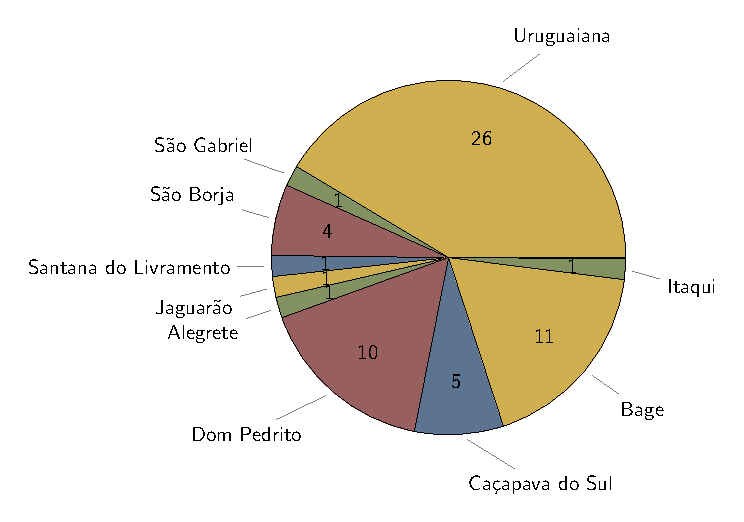
\includegraphics[width=16cm]{img/uruguaiana.pdf}
  \end{center}
  \fonte{Adapted from \cite{relatorio-2017}}
\end{figure}

%==============================================================================
Em relaçao ao tamanho mínimo da amostra, tamanhos entre 100 e 150 respondentes já seriam suficientes, pois além das respostas quantitativas teriam todas as respostas qualitativas com sugestões e melhorias, demandando mais tempo para análise.
%==============================================================================

%==============================================================================
A separação da amostra é um ponto essencial para a melhor eficiência do survey, estando de acordo com a prática recomendada 22 definida por \citeonline{Jefferson}, em que diz que a amostra deve ser dividida de acordo com as suas caracteristicas e semelhanças. 
Para contemplá-la, os respondentes do questionário que se declarassem como \acp{TAE} ou docentes eram direcionados para uma área do questionário, e discentes para outra, ambas as áreas com perguntas relacionadas ao perfil reclarado pelo respondente.

%==============================================================================
\subsection{Design and Write the Questionnaire} \label{sec:survey-questionnaire}

% (kasunic) objetivos e caracteristicas da sample para fazer o questionario, importancia dos dois
% (guideline) resultados dependem da qualidade das perguntas

% (kasunic) 4 tipos de perguntas, colcoar as que se encaixam em cada uma
% (kasunic) close ended e open ended questions 52, todas sao ordinal responses usando MoSCoW

% Colocar o questionario em apendice
%==============================================================================
\citeonline{kasunic2005designing} ressalta que para a estruturação e escrita do questionário, os objetivos de pesquisa e as características da amostra devem ser levados em conta. 
De acordo com o autor, questionarios que não possuem objetivos bem definidos tem mais chances de possuirem perguntas que só consomem tempo do respondente, ele ressalta isso com uma pergunta \citeonline[p.34]{kasunic2005designing} ``How can you reach insightful conclusions if you do not know what you were looking for or planning to observe?'', neste questionário o objetivo é bem definido, focado em priorização de requisitos e levantamento de sugestões pelos possíveis usuários finais como bem descrito na \Cref{sec:survey-objectives}. 
Da mesma maneira, as caracteristicas da amostra são importantes para escrever as perguntas de um modo que todos entendam e não apenas pensando no entendimento dos proprios pesquisadores. 
% \citeonline[p.23]
\citeonline{surveyGuidelines} atenta que os resultados que serão obtidos com o survey, estão diretamente relacionados com a qualidade do questionário utilizado.
%==============================================================================

%==============================================================================
Para \citeonline{surveyGuidelines} existem dois tipos de questionários, self-administrated and interviewer-administrated questionnaire, de acordo com suas definições este se encaixa no primeiro tipo, pois por ser um questionario web-based, não é necessário ao acompanhamento dos pesquisadores. 
Este modelo permite a maior abrangência de respondentes, mas por outro lado tende a maior taxa de desistência, ressaltando a importância de uma boa estruturação.
%==============================================================================

%==============================================================================
Para a realização do survey, foi escolhida a ferramenta do Google Forms, já que ela contribui com uma interface simples e de facil entendimento, logo que esta já é utilizada pela maioria dos perfis dos respondentes.
%==============================================================================

%==============================================================================
A estrutura do questionário que está contido no \Cref{annex:questionnaire} se da pela página inicial, questões de perfil do respondente, questões de priorização de requisitos e por fim sugestões de funcionalidades, estas estão descritas a seguir em suas respectivas seções.
%==============================================================================
\subsubsection{The Welcome Screen}
%==============================================================================
% \citeonline[p.65]
Seguindo instruções de \citeonline{kasunic2005designing}, a primeira página do questionário contém informações importantes para o participante como:

%==============================================================================

%==============================================================================
\begin{itemize}
  \item O objetivo da pesquisa;
  \item Duração estimada do questionário;
  \item Endereços de email para contato;
  \item Pesquisadores envolvidos;
  \item Caráter voluntário, anônimo e confidencial da pesquisa;
  \item Instituição e organização envolvida.
\end{itemize} 
Por fim perguntando para o participante se ele aceita em continuar com a pesquisa.

%==============================================================================

\subsubsection{Profile Questions}\label{survey:profile-questions}
%==============================================================================
As questões referentes a adiquirir informações sobre o participante são importantes nas primeiras fases do questionario, pois motivam os participantes a continuar respondendo-o sem confundi-los com perguntas complexas logo no começo, \cite{LMRea}. Além que com uma boa classificação de participantes, permite que a analise destes seja feita de maneira mais controlada e organizada como bem mencionado por \citeonline{legramante}.
%==============================================================================

%==============================================================================
Os dados que foram retirados com as perguntas de perfil, são listadas a seguir:
\begin{inparaenum}[(1)]
  \item Se o participante faz parte da \ac{UNIPAMPA};
  \item Sexo do participante;
  \item Faixa etária;
  \item Formação acadêmica;
  \item Se o participante ja esteve em alguma atividade extensionista;
  \item Se a anterior for verdadeira, quais papeis ele desempenhou;
  \item Papel do participante na comunidade acadêmica;
  \item Campus/Cidade do participante;
  \item Curso em que esta relacionado.
\end{inparaenum}
%==============================================================================

\subsubsection{Requisites Priorization Questions}
%==============================================================================
Nas perguntas relacionadas ao objetivo da pesquisa foram utilizados alguns direcionamentos descritos por \citeonline{forza}, são eles:
% \citeonline[p.168]
\begin{description}
  \item \textbf{Suggestion 1.} Define the way questions are asked to collect the information on a specific concept;\label{suggestion:1}
  \item \textbf{Suggestion 2.} For each question decide the scale on which the answers are placed;\label{suggestion:2}
  \item \textbf{Suggestion 3.} Identify the appropriate respondent(s) to each question;\label{suggestion:3}
  \item \textbf{Suggestion 4.} Put together the questions in questionnaires that facilitate and motivate the respondent(s) to respond.\label{suggestion:4}
\end{description}
%==============================================================================

%==============================================================================
Em se tratando do \textbf{Suggestion 1}, onde é sugerido que as perguntas estejam escritas de maneira que toda a amostra respondente consiga entender e formular uma resposta. 
Já que as perguntas deste questionario se referem a requisitos de software, foi utilizado o modelo de estórias de usuário, em que deixa bem explícito qual o ator, o que se deseja com o determinado requisito e o seu motivo. 
Também foi determinado que as perguntas seriam classificadas como closed questions, que determinam as possíveis respostas do respondente como descrito por \citeonline{forza}. 
Assim, no final de cada página do questionário também continha uma questão open-ended permitindo o respondente dissertar da maneira que bem entender.
%==============================================================================

%==============================================================================
A \textbf{Suggestion 2} se trata da escala utilizada nas perguntas, em um primeiro momento pensou-se em utilizar a escala Likert, mas melhor pensado posteriormente decidiu-se utilizar a escala \ac{MoSCoW}, sendo as possíveis respostas as já presentes no seu próprio nome. 
Ela foi escolhida porque esta mais relacionada a requisitos e serve justamente para a priorização de requisitos de software.
%==============================================================================

%==============================================================================
Em seguida na \textbf{Suggestion 3}, sugere-se que o questionário direcione os participantes para as perguntas que eles possuam mais propriedade para respondê-las, trazendo respostas mais construtivas e relevantes. 
No questionário utilizado, esta divisão esta sendo feita utilizando as perguntas de perfil comentadas na \Cref{survey:profile-questions}, sendo o participante automaticamente direcionado para a seção correspondente com seu perfil.
%==============================================================================

%==============================================================================
Por fim, na \textbf{Suggestion 4} é aconselhado que todas as perguntas que tem um assunto em comum, sejam organizadas próximas umas das outras para facilitar as verificações cruzadas entre as respostas. 
Para implementar esta sugestão, os requisitos estão agrupados por papéis conforme os atores do sistema, sendo eles: 
\begin{inparaenum}[(1)]
    \item Proponente de atividade de extensão;
    \item Instrutor de atividades de extensão;
    \item Coordenador de projetos ou programas de extensão;
    \item Participante de atividades de extensão.
\end{inparaenum}
%==============================================================================
\subsubsection{Feature Suggestions}
%==============================================================================
Para a última página do questionário foi disponibilizado um campo em que os respondentes podem sugerir aos pesquisadores qualquer melhoria, funcionalidade, correção etc. Com estas respostas é possível fazer uma analise qualitativa e conseguir novas ideias para o desenvolvimento e completude da ferramenta final.
%==============================================================================
\subsection{Pilot Questionnaire}\label{sec:survey-pilot}
%==============================================================================
Após ser gerado uma versão estável do questionario, é necessário validá-lo, para isto foi realizado um questionário piloto. 
% \citeonline[p.75]{kasunic2005designing} 
De acordo com \citeonline{kasunic2005designing} a pilot test is a simulation of the real questionnaire carried out with a small number of members from the target audience. 
Para realizá-lo foram escolhidas 7 (sete) pessoas, divididas em: 4 (quatro) alunos de graduação, 2 (dois) professores da \ac{UNIPAMPA} campus Alegrete e 1 (um) \ac{TAE}. 
A escolha dos respondentes do questionario piloto se deu porque ela representa todos os perfis esperados na target sample, e representa a proporção esperada na realização real do questionario.
%==============================================================================

%==============================================================================
Dos escolhidos para a participação do questionário piloto apenas um não conseguiu respondê-lo a tempo, este foi o \ac{TAE}, mas isto no final não foi um problema pois como mencionado na \Cref{sec:survey-sampling}, o questionário está divido em duas partes em que \acp{TAE} e docentes respondem a mesma.
%==============================================================================

%==============================================================================
Com a execução deste piloto foi possível adiquirir diversas sugestões, correções e pontos importantes para a versão final do questionário. 
Um exemplo disso, foi que um participante não se sentiu confortável expondo a sua idade exata, então foi sugerido que esta fosse solicitada utilizando faixas etárias.
%==============================================================================
\subsection{Distribute the Questionnaire}\label{sec:survey-distribute}

O questionário foi distribuído para todas as pessoas que compõem a amostra desta pesquisa. 
Para isto ser executado, primeiro foi realizado uma pesquisa para levantar todos os emails de coordenadores de projetos ou programas de extensão de todos os campus da \ac{UNIPAMPA}, sendo eles os primeiros a responder as respostas do questionario. 
Após 2 (dois) dias, foi enviado emails para todas as secretarias academicas dos campus, solicitando que fosse repassado para todos os seus alunos de todos os cursos. 
Concluindo, ao todo o survey ficou aberto para respostas por 18 (dezoito) dias.

\subsection{Analyze the Results and Write a Report}\label{sec:survey-analyse}

Os resultados quantitativos relacionados a priorização de requisitos, devem ser coletados e organizados em gráficos para melhor entendimento e visualização dos dados. 
Assim será possível ter uma lista ordenada de requisitos que foram considerados mais importantes para os usuários finais.

Em relação as respostas qualitativas, estas serão analisadas caso a caso e se pertinente a sugestão, serão adicionadas dentro do leque final de funcionalidades ou melhorias.

\section{Threats to Validity}\label{sec:survey-threats}

% Decições, problemas, descrever como tentamos contornar a ocorrencia
% Olhar nos trabalhos para exemplos de ameaças
% Piloto, estruturação...

\section{Result Analysis}\label{sec:survey-results}

\subsection{--} % Separação dos participantes, aluno, professor, idade, campus...

\subsection{--} % Participação em algum projeto de extensão

\subsection{--} % Classificação final, graficos